\documentclass[tikz, border=3mm]{standalone}
\usepackage{tikz}
\usetikzlibrary{
    arrows.meta,         % For arrow tips
    calc,                % For coordinate calculations
    positioning,         % For arrow tips
    decorations.markings,% For placing arrows along paths
         % For coordinate calculations
}

\begin{document}
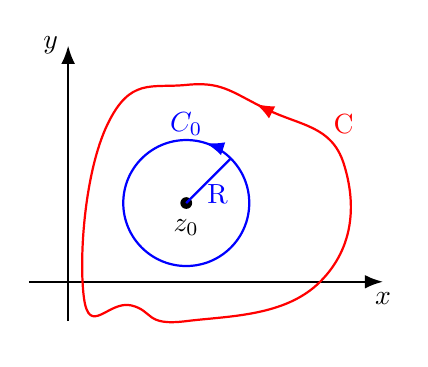
\begin{tikzpicture}[
    >=Latex, % Set default arrow tip style
    axis/.style={->, thick}, % Style for axes
    curve/.style={thick},    % Base style for curves
    dot/.style={fill=black, circle, inner sep=1.5pt}, % Style for point z0
    labelstyle/.style={}, % Base style for labels
    arrowstyle/.style={thick, shorten <=1pt, shorten >=1pt}, % Style for manual arrows
     midarrowL/.style={
        decoration={markings, mark=at position 0.2 with {\arrowreversed{Latex}}},
        postaction={decorate}
    },
    midarrow/.style={
        decoration={markings, mark=at position 0.2 with {\arrow{Latex}}},
        postaction={decorate}
    }
]

    % Axes
    \draw[axis] (-0.5, 0) -- (4, 0) node[below] {$x$};
    \draw[axis] (0, -0.5) -- (0, 3) node[left] {$y$};

    % Define center and radius for inner circle
    \coordinate (z0) at (1.5, 1.0);
    \def\radius{0.8};

    % Define coordinates for outer blob C (adjust as needed)
    \def\coordsOuter{
        (0.2, -0.2) % Bottom left
        (0.5, 2.0)  % Mid left
        (1.5, 2.5)  % Top middle
        (2.5, 2.2)  % Top right
        (3.5, 1.5)  % Mid right
        (3.2, 0.0)  % Bottom right
        (1.5, -0.5) % Bottom middle
        (0.8, -0.3) % Bottom leftish
    }

    % Draw Outer Red Blob (C)
    \draw[curve,midarrowL,  red] plot [smooth cycle, tension=0.8] coordinates {\coordsOuter};
    \node[red] at (3.5, 2.0) {C}; % Label C

    % Draw Inner Blue Circle (C0)
    \draw[curve, midarrow, blue] (z0) circle (\radius); % Draw circle border
    \node[blue] at ($(z0)+(90:\radius+0.2)$) {$C_0$}; % Label C0 above circle

    % Draw Center Point z0
    \node[dot, label={[labelstyle, black]below:$z_0$}] at (z0) {};

    % Draw Radius Line and Label R
    \coordinate (R_end) at ($(z0)+(45:\radius)$); % Endpoint on circle at 45 deg
    \draw[blue, thick] (z0) -- (R_end);
    \node[blue, below=1pt] at ($(z0)!0.7!(R_end)$) {R}; % Label R along the line

    % --- Manual Arrows ---
    % Arrow for Outer Curve C (Red, CCW) - Place near left side
    \coordinate (Carrowpos) at (0.5, 2.0); % Point on curve
    % Draw arrow tangent-like (pointing up-right for CCW)
   % \draw[->, arrowstyle, red] ($(Carrowpos)+(-0.1,-0.1)$) -- ($(Carrowpos)+(0.1,0.1)$);

    % Arrow for Inner Circle C0 (Blue, CW) - Place near left side (angle ~135 deg)
    \coordinate (C0arrowpos) at ($(z0)+(135:\radius)$);
    % Draw arrow tangent-like (pointing down-right for CW)
  %  \draw[->, arrowstyle, blue] ($(C0arrowpos)+(-0.1,0.1)$) -- ($(C0arrowpos)+(0.1,-0.1)$);
    % --- End Manual Arrows ---

\end{tikzpicture}
\end{document}